\chapter{General discussion and
recommendations}\label{ch:conclusions}
\section{Introduction}

The principal objective of this thesis has been to characterise
the Galician shelf response to the varying seasonal forcing, in
particular to identify the typical spatial and temporal
variability of wind and its effect on the shelf circulation.
Through a set of observations including satellite data
(scatterometer, AVHRR, SeaWIFS and drifters), cruise data (CTD,
ADCP, turbulence probe) and mooring data (wind and surface
currents) the complex shelf circulation and its response to large
scale forcing has been explored. Many of the observations,
although limited in their spatial and temporal coverage, are novel
in an area where systematic sampling has been sparse. In
Chapter~\ref{ch:winds}, for the first time, the spatial and highly
temporal variability of the wind has been unequivocally shown and
indirect evidence of its effect, through SST has been presented.
Results from Chapter~\ref{ch:winds} were extrapolated to help the
interpretation of SST data in the absence of direct spatial wind
measurements. In subsequent chapters, examples of the spring
transition, upwelling season and autumn transition/downwelling
stage have been presented covering the contrasting shelf
environments identified for the Galician CTZ in the literature.
The last chapter provided an integrated quantitative view of the
Lagrangian differences between the upwelling and downwelling
regime.

\section{Shelf classification} The gently sloping shelf around
Galicia extends, on average, 40km seawards either side of Cape
Finisterre (with a minimum at the Cape of 20km) constituting a
narrow shelf.  Even in the absence of filament formation, the
upwelling front extends beyond the shelf break into waters
$>$1000m (Chapter~\ref{ch:winds}). This is expected during
sustained favourable upwelling winds in a wide shelf, or for a
narrow shelf with intermittent upwelling winds, as in Galicia. The
front's offshore position is an indication of weak topographic
control, as the shelf break would anchor the upwelling front
there, in contrast with the stronger link reported by
\citet{Fiuza96b} and \citet{Peliz02} in the wider Portuguese shelf
south of 41\deg (Figs~\ref{fig:largebathy}
and~\ref{fig:summerupw}c). There, the upwelling front resembles
the geometry of the bottom topography. Upwelling areas very often
have associated poleward undercurrents \citep{Neshyba89,Barton90}
which in narrow shelves are located off-shelf. This is the case in
the Galician region, where the poleward flowing Portugal Coastal
Under Current (PCUC) is located on the slope during strong
upwelling wind episodes
(Chapters~\ref{ch:spring}-\ref{ch:summer}). The shelf can be
expected to function like a shallow one, with surface and bottom
Ekman layers occupying the entire water column in a two layer
circulation \citep{Garvine71,Hill98}. It is only during wind
relaxations (Chapter~\ref{ch:summer}) that the poleward
undercurrent occupies the shelf.

The small width of the shelf means there is a strong interaction
between the shelf circulation, the circulation inside the Rias and
the wind forcing. Previous authors have acknowledged this for the
Rias Bajas \citep[e.g.][]{Gomez-Gesteira01,Prego01,Sordo01} and
they have to be considered an integral part of the shelf in as
much as it responds to the same forcings. Upwelling and
downwelling winds greatly modify the circulation inside the Rias,
enhancing or reducing their flushing time throughout the year,
even during maximum river runoff in autumn and winter
\citep{Alvarez-Salgado00}. During the summer the river discharge
is minimum, but upwelling takes place inside the Rias where
upwelled water undergoes warming, freshening and nutrient
utilisation. The effect of outwelling from the Rias on the shelf
circulation is greatest in the presence of the PCC
(Chapter~\ref{ch:spring}), as the freshwater plume can reach the
shelf break and interact with the PCC. The enhance stratification
on the shelf could potentially delay the outcropping of the
isothermals.


\section{Variability} It has been shown that the upwelling region
of Galicia is a highly variable system. Two main interconnected
sources of variability have been identified in the present work:
the irregular coastline and shelf with its major example in Cape
Finisterre, and the strong variability at spatial and temporal
scales of the wind forcing. Both aspects affect the development
and evolution of the upwelling regime (Chapter~\ref{ch:winds}) as
also shown for the Oregon coast by \citet{Barth00,Samelson02} and
the downwelling regime (Chapter~\ref{ch:drifters})
\citep[e.g.][]{Dubert98}. Small Time scales have been consistently
obtained from Lagrangian observations and large scale winds and
hint at a very dynamic region. Despite its complexity, the
mesoscale wind variability can be reduced to a finite number of
spatial patterns which, to a first approximation, explain the
Galician shelf response (Chapter~\ref{ch:winds}). One quarter of
the wind spatial variability rests in increasingly complex spatial
patterns, while three quarters correspond to a coherent wind. The
seasonality of the wind forcing is masked by upwelling/downwelling
events throughout the year as also noted in previous studies
\citep{Alvarez-Salgado03}. However, the system response shows a
clearer seasonality with upwelling during the summer and
downwelling during winter mediated by a meridional density
gradient. It is the more consistent and frequent upwelling winds
during the summer that determine this seasonality. However, the
intermittency of upwelling winds (Time scales of 14 days,
Chapter~\ref{ch:winds}) produce a contouring broad upwelling front
(Chapter~\ref{ch:summer}, Fig~\ref{fig:cd114_shelftran})
\citep{Brink83} rather than the sharp one measured south in the
broader Portuguese shelf \citep{Peliz02}. Each upwelling pulse
would generate a new front that will be advected offshore and
modified by surface heating and freshwater mixing. Further south,
along the Portuguese coast, the wind is expected to be stronger
and less variable similar to Oregon-California differences, as a
result of the continental mass and coastal guidance. Nonetheless,
interannual differences in the upwelling and downwelling regimes
are large \citep{Huthnance02} and related to the wind. Unusual
predominance of PUNC over PUWC patterns restrict filament
development on the west coast while enhancing the Cape Finisterre
filament as was the case in 1999 (Chapter~\ref{ch:winds}).
Integrated values of monthly upwelling indices for the west coast
(Vigo region, as in Chapter~\ref{ch:spring}) showed smaller values
in 1999 (119 \Eidx) compared to 1998 (273 \Eidx) when west coast
filaments fully developed (Chapter~\ref{ch:summer}), which agrees
with the expected differences between ``PUNC'' and ``PUWC'' years.
Similarly, predominance of PUWC patterns over DOWN patterns during
the winter of 1999 precluded the development of the poleward flow
over the slope (Chapter~\ref{ch:drifters}).

Rather than long upwelling index integrals (i.e. over the summer
months), \citet{Austin02} found that a finite integration between
5-12 days, best explained the upwelling intensity measured as the
displacement from horizontal (outcropping) of the permanent
pycnocline. If this holds for the Galician region given the
similarities in wind forcing, the characteristic wind time scale
of 14 days would suffice to maintain an active and productive
upwelling. \citet{Austin02} also found that a wind relaxation of
5-12 days produced a dynamical relaxation stage, i.e. the
pycnocline relaxed but still produced a southward geostrophically
balanced jet. The relaxation process can be driven by alongshore
pressure gradients created during upwelling events \citep{Send87}
or alongshore variations in wind stress \citep{McCreary87} among
other mechanisms. Alongshore variations in upwelling conditions
may lead to alongshore transport divergence and hence regions of
high or low pressure, and the opposing pressure gradients drive
alongshore poleward flow. This alongshore flow, in turn, drives
transport in the bottom Ekman layer counter to that in the bottom
Ekman layer during the wind event which would restore the density
structure to a more horizontal position. \citet{Samelson02}, in
their study of wind scatterometer data off the coast of Oregon,
have shown a systematic increase of southward wind stress by a
factor of 3-4 along the Oregon coast. Whether such a wind
variation can be expected off the Iberian coast remains to be
assessed although some indications can be seen in the median of
wind during the summer 1999 and 2000 in Fig~\ref{windsmedian} and
in the reconstructed wind patterns (Fig~\ref{fig:windsreconfig}).
Nonetheless, the latitudinal variation in the upwelled watermass
characteristics could also induced alongshore pressure gradients.
The latitudinal variation of density in the upwelled waters shown
in Chapter~\ref{ch:litrev} (Fig~\ref{fig:litts}) represents 1\dens
change in 500km, a gradient of $\sim 10^{-6}$\dens per m,
sufficient to drive a poleward flow (Chapter~\ref{ch:winter}).
This could account for the existence of the PCUC seen during the
relaxation event in Chapter~\ref{ch:summer}.

With no clear seasonal wind changes in the scatterometer data the
transitional periods between downwelling and upwelling regimes are
difficult to examine. Monthly upwelling index
(Chapter~\ref{ch:summer}) suggest a mean long spring transition
(April to June) from the downwelling to upwelling regime for the
1986-1998 record, due to high wind variability. During those
months, co-existence of the PCC and coastal upwelling is possible
(Chapter~\ref{ch:spring}). However, upwelling relaxations or
downwelling winds quickly suppress the coastal upwelling (e.g.
Chapter~\ref{ch:winds}). These early upwelling events are eroded
faster because the upwelled water does not provide a strong
upwelling front or sea level declining onshore in response to high
density water. The compensatory onshore flow originates from above
the bottom Ekman layer of the poleward flow with watermass
characteristics similar to the surface water. Upwelling is not
permanently established until the poleward flow shuts down or is
pushed offshore.

Interannual and seasonal variability of the large scale
circulation influences the development of the poleward flow. The
seasonal signal in the Sea Level Anomaly (SLA), as determined from
altimetry data for 1992-1998, is large offshore the Iberian
peninsula \citep{Efthymiadis02}, and is related to changes in the
upper-ocean heat content. The authors found maximum negative SLA
during autumn and winter, enhancing the southward flowing Portugal
Current, in part responsible for the maintenance and
intensification of the meridional density gradient off Iberia that
drives the PCC. \citet{Martins02} have shown a seasonal increase
in altimetry derived altimetry Eddy Kinetic Energy (EKE) from
autumn, maximum in winter, and decreasing towards the summer in
the region of the Portugal Current for 1992-1999. The increase is
partly related to the higher number of eddies in the region of the
meridional density front. Both SLA and EKE seasonal trends are
related; the enforcement of the Portugal current sharpens the
front, which allows for eddy formation, which at times, could help
maintain and enhance the front as discussed by \citet{Dubert98}.
Both mechanisms reinforce the slope poleward flow but also cause
pulses as eddies could modulate the impingement of the front on
the slope.

Interannual variability was seen in both EKE\citep{Martins02} and
SLA \citep{Efthymiadis02} off Iberia. The dominant interannual
basin scale variability during winter over the North Atlantic is
the North Atlantic Oscillation (NAO) \citep{Rogers85}. The NAO
index is defined as the normalised sea-level pressure difference
between the Azores and Iceland \citep{Jones97} and it is
associated with changes in the strength and direction of winter
westerly winds over the North Atlantic and northwest Europe.
Winter negative NAO values correspond to stronger westerly winds
on the subtropical North Atlantic. It is not surprising then that
interannual variations matching the NAO index are more dominant
north of 34\deg N \citep{Efthymiadis02} and are greater during the
winter related to the wind-induced net heat loss. \citet{Garcia02}
studied the relationship between the NAO index and the presence of
the PCC along the Bay of Biscay and found a good relationship
between winter negative NAO index and strong poleward flow
development. \citet{Efthymiadis02} found the largest SLA fall
during 1995/96, which corresponded to strong poleward flow
development year \citep{Garcia02,Pingree99}. 1999 was a year of
positive NAO index which relates to weak downwelling/upwelling
winds during winter off Iberia and the PCC failed to develop
(Chapter~\ref{ch:drifters}).

The year around presence of a poleward flow in the Galician CTZ
has been suggested previously, switching from the winter surface
flow (Chapter~\ref{ch:winter}) to an undercurrent one during the
summer upwelling (Chapter~\ref{ch:summer}), but direct
observational evidences are sparse \citep{Barton90}. Here, two
different forcing mechanisms are proposed for the PCC and the
undercurrent. The adjustment process of the meridional oceanic
density gradient to the slope-shelf topography drives the PCC
while an alongshore pressure gradient induced by the latitudinal
variation of the watermass characteristics of the upwelled water
forces the undercurrent.

\section{Seasonality} An schematic of the expected upper layer seasonal
circulation in the Galician shelf is proposed in
Fig~\ref{fig:concl_sketch}.
\subsection{The downwelling or poleward flow regime}
The poleward flowing PCC undergoes a development phase during
which the meridional density gradient strengthens in late autumn
and early winter. The current develops the typical narrow
tongue-like structure off Galicia broadening north of Cape
Finisterre (Fig~\ref{fig:concl_sketch}a). The shelf is effectively
isolated from the ocean due to the shelf-edge front
(Chapter~\ref{ch:winter}) although some exchange takes place in
the form of a bottom Ekman layer. Finally it reaches a
mature/turbulent stage with eddies pitching off albeit with
limited export capabilities \citep{Huthnance02}. In this respect,
horizontal diffusivities were smaller when compared to estimates
during the upwelling regime (Chapter~\ref{ch:drifters}). Cape
Finisterre and Cape Ortegal have been suggested as the possible
origin of both SWODDIES \citep{Pingree92} and MEDDIES
\citep{Paillet02}. The PCC transports \enawt northward and its
chemical signature changes downstream. In particular, off Iberia,
the mixing between the PC and the PCC accounts for the northward
indirect ventilation (increase in oxygen and decrease of
nutrients) of \enawt by the \enawp transported in the PC
\citep{Perez01}. The distinctive biogeochemical signature of the
PCC has a large impact on the biology of the shelf as shown by
\citet{Alvarez-Salgado03} affecting the timing of the autumn and
spring bloom, the phytoplankton assemblages and the carbon export
between the shelf and the ocean.

\begin{figure}
\centering \arribacap%
\subfigure[]{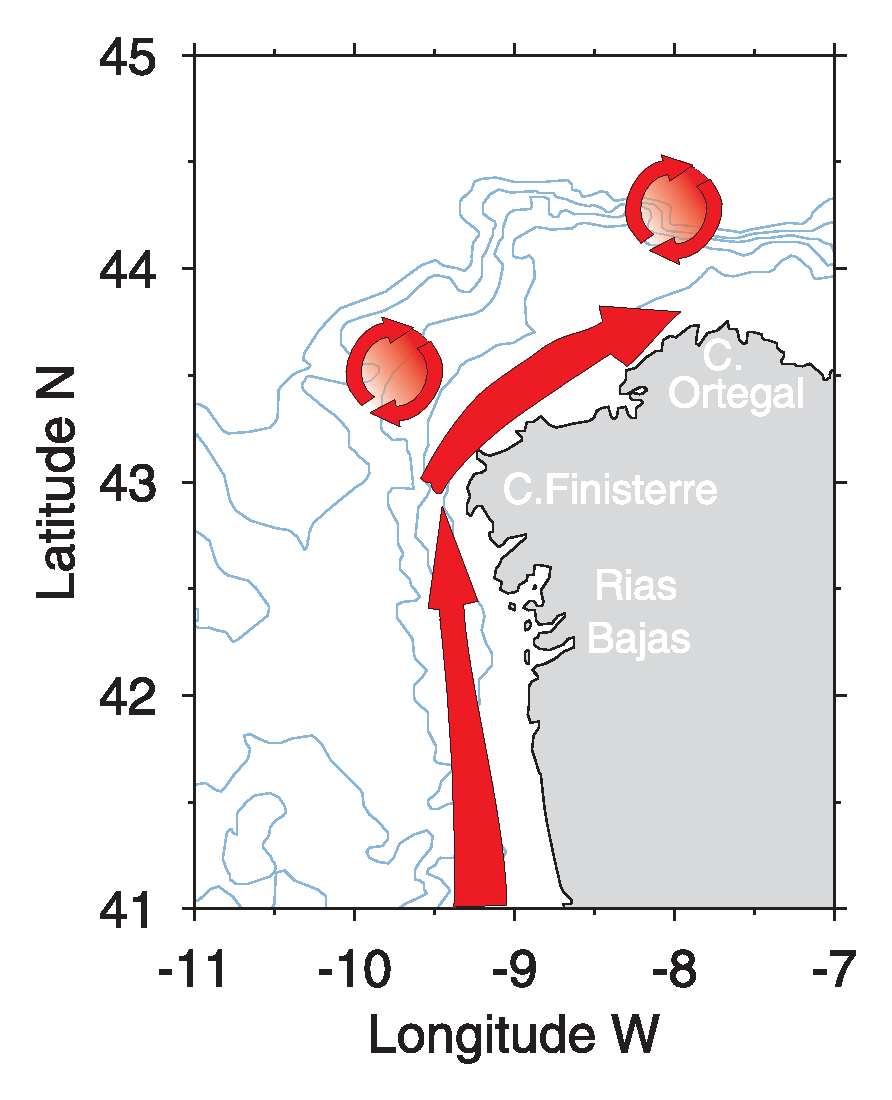
\includegraphics[width=7cm]{wintercircfinal}}%
\subfigure[]{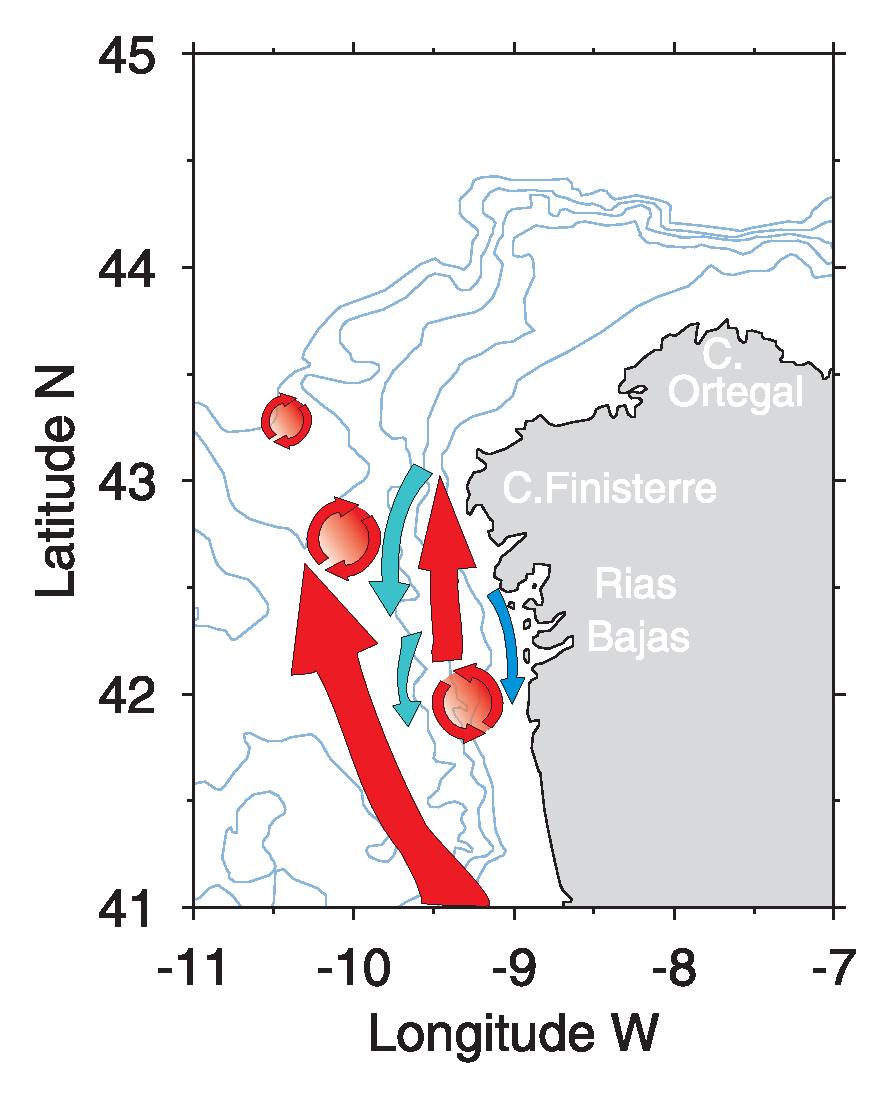
\includegraphics[width=7cm]{springcircfinal}}
\subfigure[]{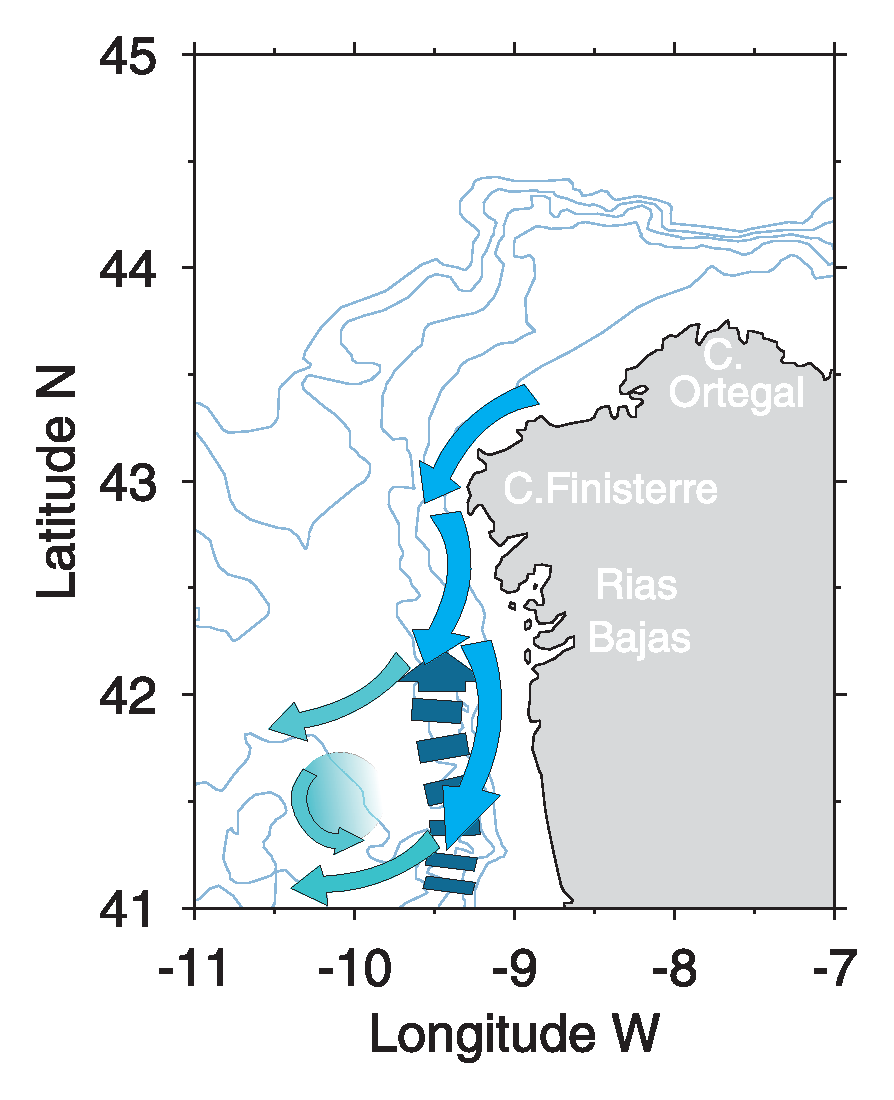
\includegraphics[width=7cm]{summercircfinal}}%
\subfigure[]{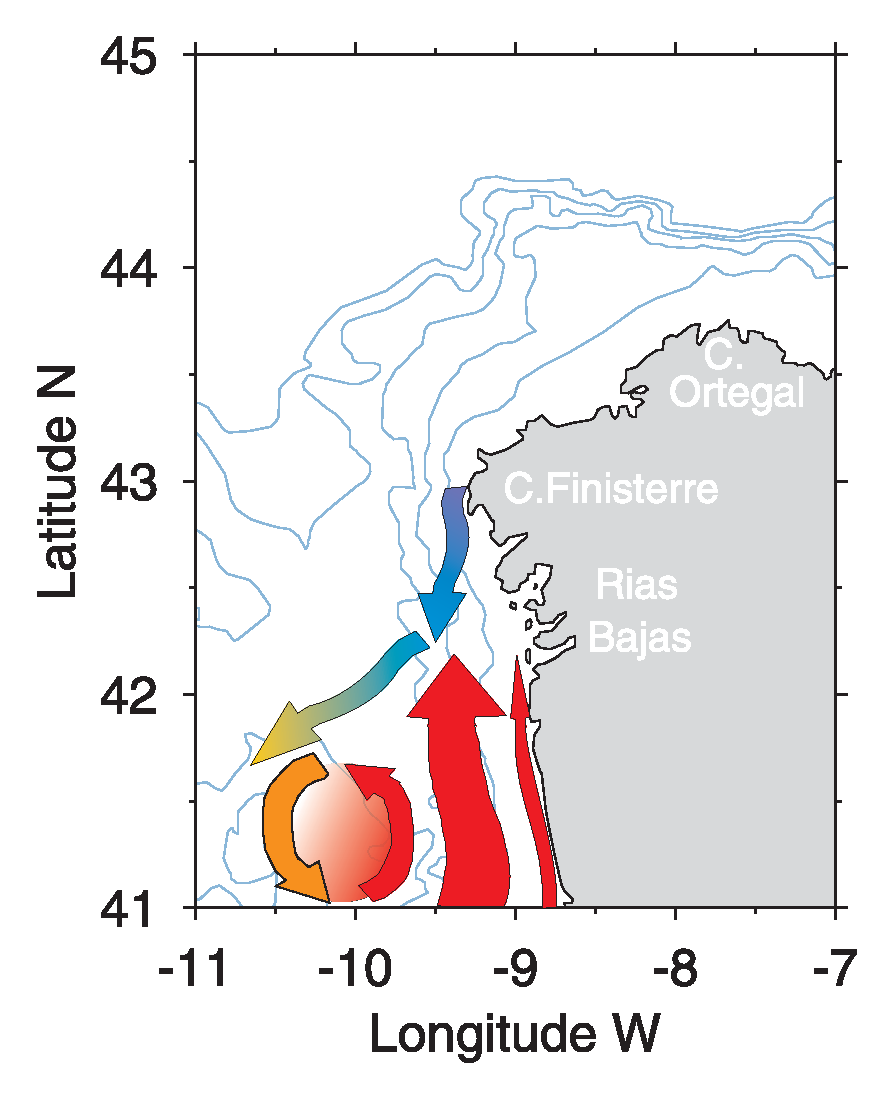
\includegraphics[width=7cm]{autumncircfinal}}
\caption{Schematic of the surface (solid arrows) and subsurface
(broken arrows) circulation during (a) winter, (b) spring, (c)
summer and (d) autumn. A colour scheme is used were red
corresponds to warmer temperatures and green/blue to cooler ones.
See text for details } \label{fig:concl_sketch}
\end{figure}

\subsection{The transition between downwelling to upwelling regime}
The weakening of the meridional density gradients sparks the decay
phase of the poleward slope current. The PCC was still present in
June 1997 prior to the onset of coastal upwelling
(Chapter~\ref{ch:spring}). Upwelling favourable winds push the
flow offshore establishing a second northward flow offshore. At
this late stage, the PCC was better established offshore than on
the slope, which has by now broadened, and distorted by
interactions with the mesoscale eddy field
(Fig~\ref{fig:concl_sketch}b). A portion of the PCC is still
depicted on the slope south of Cape Finisterre as the main
detachment point is off the Rias Bajas. The upwelling winds
quickly establish a southward flowing jet nearshore while a second
southward flow separates the two PCC branches. A similar southward
flow intrusion separating general northward flow was also measured
by \citet{Almeida99} at the end of the upwelling season near Cape
Sa\~o Vicente, south of Portugal. The author related it to a
remnant of the coastal upwelling front. In our case, the upwelling
regime had not been established yet and it is more likely the
result of advection of colder oceanic water from off Cape
Finisterre by the two eddies seen in the velocity data
(Chapter~\ref{ch:spring},
Figs~\ref{fig:cd105_51m}-~\ref{fig:cd105_100m}).

\subsection{The upwelling regime}
During the upwelling regime, the upper column structure becomes
dominated by coastal upwelling and filaments and the poleward flow
is restricted to deeper levels (Fig~\ref{fig:concl_sketch}c). As
discussed previously, there is a strong interannual variability
during the upwelling regime characterised by either
presence/absence of filaments on the west coast or whether the
main filament is at Cape Finisterre or at 42\deg latitude.
Nonetheless, coastal upwelling was present in all years studied
here. This supports the idea of growing instabilities associated
with the upwelling front as suggested by \citet{Hanyes93} and
\citet{Roed99}. An eddy field would generate filaments whenever an
upwelling front is present. In Fig~\ref{fig:concl_sketch}c it is
shown a schematic of the mature stage of west coast upwelling. Up
to two filaments can be present at this stage, one rooted at
42\deg N and another one at 41\deg N. The latter was more
intermittent and can shift its position northward and merge with
the 42\deg N one (Chapter~\ref{ch:summer}). Although weak,
upwelling can still be seen north of Cape Finiterre. Detailed
\emph{in situ} sampling of the 42\deg N filament revealed  a very
shallow structure which might only be representative of a decaying
structure or typical of the Galician upwelling regime. The export
capabilities of the filaments were small
(Chapter~\ref{ch:summer}), not only due to its relatively weak
offshore transport within the filament, but also due to the
filament return flow. Although diffusive transport was enhanced
during the summer upwelling regime it was still small compared to
other upwelling areas (Chapter~\ref{ch:drifters}).

\subsection{The transition between upwelling to downwelling
regime} Towards the end of the upwelling regime, when the
upwelling winds start weakening, the poleward flow climbs back
onto the upper slope
(Chapter~\ref{ch:winter},Fig~\ref{fig:concl_sketch}d). The
meridional density strengthens possibly through the seasonal
intensification of the  Portugal current and the poleward flow
surfaces again. If filaments are still present, the offshore end
is broad, badly defined and bents southward describing a short
lived eddy like closed circulation (Chapter~\ref{ch:summer}). The
slope poleward flow eventually cuts their water supply as it
progresses northward and they slowly mix away.

The Coastal countercurrent, briefly discussed in
Chapter~\ref{ch:summer} is clearly visible in years of high
filament activity. Similar nearshore poleward flows have been
reported for the California Current System \citep[e.g.][]{Send87}
and related to a poleward pressure gradient caused by cape induced
wind-curl and subsequent wind relaxation events \citep{Wang97}. In
this case, there is no major cape associated with the poleward
coastal current and the alongshore variability might originate
from the filaments and/or freshwater plume dynamics
\citep[e.g.][]{Peliz02} and drive the shelf poleward flow during
upwelling relaxations.

\section{Future work}
Although there have been various significant efforts to observe
facets of the Galician or Iberian upwelling over the years e.g.
recently MORENA, OMEX II, there has never been a systematic effort
to monitor its year-round physical development with simultaneous
hydrographic, current and meteorological observations on the scale
of the California Current programs like CUEA or CODE. The
gradualist approach, while it has illuminated many aspects of the
system, has left many basic questions like the 3-d structure, the
spin up and spin down of upwelling, the importance of alongshore
propagating upwelling signals, unanswered. The latest oil spill by
the tanker Prestige in Galicia has highlighted the need for
further understanding of the oceanography of the region.

The current study has focused on the Galician shelf, however, the
Iberian upwelling system encompasses the entire Portugal shelf and
subsequent studies should address the connection and feed back
mechanisms over the whole system. For example, the large scale
wind field and its temporal variability needs to be characterised
including any spatial trends as found in the California-Oregon
coast and possible remote forcing signals. On a more regional
scale, intensive and extensive sampling of the region response to
north/west coast upwelling should clear its effect on the system
evolution. The local effect of the prominent Finisterre filament
has been speculated but detailed studies of small scale shelf
circulation and the wind distribution around the Cape should help
understand and quantify its effect. Such detailed studies could
also address the open questions about the response of the Rias
circulation to both wind and shelf circulation and the possible
feedback mechanisms as would the effect of small topographic
features like canyons at the shelf edge on the upwelling system.

The results from the \emph{in situ} survey of the 42\deg N
filament were quite surprising and further detailed sampling of
the 3-D filament structure are needed in order to provide a more
accurate description of its dynamics and assess the relevance of
the results presented here. Evidences pointing at the year around
presence of a poleward undercurrent have been presented but future
efforts should be directed at the forcing mechanisms particularly
during the upwelling regime. Current knowledge regarding the
dynamics and  driving forces of the poleward coastal
countercurrent are scarce and giving its economic impact (e.g. its
relation to HAB events in the Rias Bajas, one of the world largest
producer of mussels), its study is a pressing matter.

The poleward winter flow (the PCC) has received a good deal of
attention in the last decade but mostly from remote sensing and
only a handful of studies have surveyed the feature \emph{in
situ}. A more intensive study of the poleward flow, both at a
large scale looking at the variability of the large scale
circulation and its dependency on the wind forcing, and joint
modelling and \emph{in situ} regional studies should clarify its
interannual variability and should unequivocally show the main
source of the variability and quantify the effect of the wind
forcing in precluding its year around presence.

Coastal Trapped Waves (CTW) role in the system's evolution and
other high frequency sub-inertial signals. CTW could be of
importance given the large wind variability. \citet{Huthnance02}
reported that 4-6 day wind stress fluctuations excited a
second-mode CTW with 4-6 day current fluctuations which
corresponded to a phase speed of 2.2\vel.

The prominent location of the Galician region in relation to
marine traffic and its dangerous waters (there have been more oil
spills in the last 25 years than in any other European waters)
requires efforts to be directed towards an operational
oceanography strategy. For it to be successful, data are needed to
validate models and design measurement networks to maximise
resources.

Many of these questions could partially be tackled from a
modelling point of view. However, existing modelling efforts on
the region have been restricted to climatological experiments and
idealised topography. The relevance shown here of the complex
topography and short time variability calls for better and more
realistic topography, coast and wind forcing.
